\chapter{Methodology}
\label{chap:methods}

\section{Research Design}
\label{sec:study_design}

This study used a comparative, descriptive design to examine how three large
vision--language model (LVLM) configurations classified the same images using
a common moral-category framework. Figure~\ref{fig:study_design} summarises the
study components and their relationship to the research questions.

\begin{figure}[H]
    \centering
    \begin{spacing}{1.0}

    \definecolor{flowNavy}{HTML}{17365D}
    \definecolor{flowBlue}{HTML}{2F6F9F}
    \definecolor{flowTeal}{HTML}{2A7F7F}
    \definecolor{flowAmber}{HTML}{A36A2D}
    \definecolor{flowViolet}{HTML}{665A9B}
    \definecolor{flowRule}{HTML}{AEB8C2}
    \definecolor{flowMuted}{HTML}{53616E}
    \definecolor{flowPale}{HTML}{F4F7FA}

    \begin{tikzpicture}[
        font=\sffamily\scriptsize,
        anchorbox/.style={
            draw=flowNavy,
            fill=flowNavy,
            text=white,
            rounded corners=3pt,
            align=center,
            text width=13.3cm,
            minimum height=1.05cm,
            inner sep=4pt
        },
        primarybox/.style={
            draw=flowBlue,
            fill=flowPale,
            rounded corners=3pt,
            align=center,
            text width=8.15cm,
            minimum height=1.25cm,
            inner sep=4pt
        },
        surveybox/.style={
            draw=flowTeal,
            fill=flowPale,
            rounded corners=3pt,
            align=center,
            text width=4.25cm,
            minimum height=1.25cm,
            inner sep=4pt
        },
        branch/.style={
            draw=flowRule,
            fill=white,
            rounded corners=3pt,
            align=center,
            text width=2.35cm,
            minimum height=3.25cm,
            inner sep=4pt
        },
        humanbranch/.style={
            draw=flowRule,
            fill=white,
            rounded corners=3pt,
            align=center,
            text width=4.25cm,
            minimum height=3.25cm,
            inner sep=4pt
        },
        flowline/.style={
            draw=flowMuted,
            line width=.7pt
        },
        arrow/.style={
            flowline,
            -{Stealth[length=2.2mm,width=1.6mm]}
        }
    ]

        \node[anchorbox] (anchor)
        {
            \textbf{SHARED ANALYTICAL BASIS}\\[.8mm]
            Fixed corpus: 127 images
            \quad$\vert$\quad
            Output vocabulary: ten study-specific moral labels plus
            \textit{None}
        };

        \node[
            primarybox,
            below=9mm of anchor,
            xshift=-2.65cm
        ] (primary)
        {
            {\color{flowBlue}\bfseries PRIMARY MODEL CLASSIFICATION}\\[.8mm]
            127 images $\times$ 3 configurations\\
            381 labels, confidence scores, and brief reasons
        };

        \node[
            surveybox,
            below=9mm of anchor,
            xshift=4.25cm
        ] (surveydata)
        {
            {\color{flowTeal}\bfseries PARTICIPANT SURVEY}\\[.8mm]
            Fixed 16-image pool\\
            56 retained responses\\
            280 Part~1 observations
        };

        \node[
            branch,
            below=12mm of primary,
            xshift=-2.75cm
        ] (core)
        {
            {\color{flowBlue}\bfseries RQ1--RQ2}\\[1.2mm]
            \textbf{COMPLETE CORPUS}\\[1.5mm]
            Label use and confidence\\[1mm]
            Agreement at 11-, 6-, and 2-outcome resolutions
        };

        \node[
            branch,
            below=12mm of primary
        ] (edits)
        {
            {\color{flowAmber}\bfseries RQ4}\\[1.2mm]
            \textbf{EDITED CASES}\\[1.5mm]
            8 base images\\
            11 variants\\[1mm]
            33 attempts\\
            32 valid matched outputs
        };

        \node[
            branch,
            below=12mm of primary,
            xshift=2.75cm
        ] (repeats)
        {
            {\color{flowViolet}\bfseries RQ2}\\[1.2mm]
            \textbf{REPEATED-RUN STABILITY}\\[1.5mm]
            Stratified 32-image subset\\[1mm]
            3 runs per model\\
            288 outputs
        };

        \node[
            humanbranch,
            below=12mm of surveydata
        ] (rq3)
        {
            {\color{flowTeal}\bfseries RQ3}\\[1.2mm]
            \textbf{PARTICIPANT--MODEL COMPARISON}\\[1.5mm]
            Participant set overlap and image-level variation\\[1mm]
            Participant inclusion of model-selected labels
        };

        \coordinate (topsplit)
            at ($(anchor.south)+(0,-4.5mm)$);

        \draw[flowline]
            (anchor.south) -- (topsplit);

        \draw[flowline]
            (primary.north |- topsplit) --
            (surveydata.north |- topsplit);

        \draw[arrow]
            (primary.north |- topsplit) --
            (primary.north);

        \draw[arrow]
            (surveydata.north |- topsplit) --
            (surveydata.north);

        \coordinate (primarysplit)
            at ($(primary.south)+(0,-5.5mm)$);

        \draw[flowline]
            (primary.south) -- (primarysplit);

        \draw[flowline]
            (core.north |- primarysplit) --
            (repeats.north |- primarysplit);

        \draw[arrow]
            (core.north |- primarysplit) --
            (core.north);

        \draw[arrow]
            (edits.north |- primarysplit) --
            (edits.north);

        \draw[arrow]
            (repeats.north |- primarysplit) --
            (repeats.north);

        \draw[arrow]
            (surveydata.south) --
            (rq3.north);

        \draw[arrow, rounded corners=2pt]
            (primary.east) -- ++(2mm,0) |- (rq3.west);

    \end{tikzpicture}
    \end{spacing}

    \caption{Overview of the study components and their relationship to the
    research questions. RQ2 combines inter-model agreement on the primary
    corpus with repeated-run stability. RQ3 combines participant response
    sets with the primary model labels.}
    \label{fig:study_design}
\end{figure}

\FloatBarrier

The primary classification provided the data for RQ1 and the inter-model
component of RQ2. Repeated classifications on a selected subset addressed the
within-model component of RQ2 by placing inter-model disagreement in the
context of within-model variation. The participant survey provided the data
for RQ3, while the matched image-edit cases addressed RQ4.

The category field supplied with the image corpus was retained only as
metadata. Neither this field nor the participant responses was used to
construct a reference standard. The primary analyses therefore focused on
classification patterns, model-reported confidence, consistency within and
between models, participant--model correspondence, and selected image-edit
cases. Across all components, the findings were interpreted as descriptive
evidence; they did not estimate accuracy against validated reference labels,
population-level model performance, or causal effects of image editing.




\section{Image Corpus and Moral Taxonomy}
\label{sec:image_dataset}

\subsection{Corpus Source and Scope}
\label{subsec:image_collection}

The study analysed a fixed corpus of 127 images supplied by the project
supervisor. According to the accompanying project-level information, 51 images
(40.2\%) were obtained from online sources and 76 (59.8\%) were generated
through the Google Gemini application \cite{google2026geminiimages}.

The project supervisor confirmed that the 51 online images were obtained from
open-source materials available for reuse. The remaining 76 images were
generated specifically for this project using Google Gemini. The corpus was
therefore analysed as a constructed stimulus set rather than as a
representative sample from a defined image population.

The supplied corpus also included one researcher-assigned category field for
each image. The available records did not establish an independent,
pre-specified multi-annotator validation or adjudication procedure. This field
was therefore retained only as descriptive metadata: model--researcher
differences were not classified as model errors and were not used to calculate
accuracy. The current frequencies in this metadata field were highly uneven:
73 of the 127 images were coded as \textit{None}, while the remaining 54 were
distributed across eight represented moral labels, with 2--14 images per label.
At foundation resolution, these 54 images comprised 26 Care/Harm images and
only five to nine images in each of the other four foundations. These
single-researcher codes were descriptive indexing metadata, not validated
reference labels or sampling strata. Consequently, marginal model output
frequencies were used only to describe the retained outputs on this fixed
corpus, not to estimate a model's general category preference or performance.

\subsection{Operational Label Framework and Resolution Mapping}
\label{subsec:category_framework}

The classification task used a study-specific operationalisation of five
foundations from Moral Foundations Theory
\cite{graham2009liberals,graham2011mapping}. Each foundation was represented by
two separately selectable task labels, yielding ten moral-category labels.
These labels were task-specific categories derived from the five foundations,
rather than ten independent moral foundations or a validated image-annotation
scale.

\begin{itemize}

\item \textbf{Care/Harm foundation.}
\textit{Care} represented concern for others' well-being, needs, or
vulnerability, including compassion, helping, nurturing, support, and
protection from harm. \textit{Harm} represented physical or emotional
suffering, injury, cruelty, abuse, violence, or actions that cause or
contribute to harm.

\item \textbf{Fairness/Cheating foundation.}
\textit{Fairness} represented concern for justice, equality, rights,
impartial treatment, fair opportunities, or equitable outcomes.
\textit{Cheating} represented violations of fairness through deception,
exploitation, rule-breaking, favouritism, manipulation, or the pursuit of
an unfair advantage.

\item \textbf{Loyalty/Betrayal foundation.}
\textit{Loyalty} represented commitment, solidarity, allegiance, or
support towards one's group or its members. \textit{Betrayal} represented
violations of trust or loyalty through disloyalty, abandonment,
deception, or acting against one's group or trusted others.

\item \textbf{Authority/Subversion foundation.}
\textit{Respect / Authority} represented respect for legitimate
authority, social roles, rules, hierarchy, institutions, social order, or
established traditions. \textit{Subversion} represented defiance,
rejection, disruption, or the undermining of legitimate authority,
established rules, hierarchy, social order, or traditions.

\item \textbf{Sanctity/Degradation foundation.}
\textit{Sanctity} represented concern for purity, sacredness, dignity,
moral integrity, or the protection of things regarded as morally,
culturally, or spiritually inviolable or worthy of reverence.
\textit{Degradation} represented violations of purity, sacredness, or
dignity through contamination, desecration, humiliation, objectification,
or degrading treatment.

\item \textbf{None of these/Not clearly moral in nature.}
This option was selected when none of the ten moral categories was clearly
supported by the visible content of the image, or when identifying a primary
moral concern would require substantial unsupported assumptions. It functioned
as an insufficient-evidence or no-clear-moral-category option and was not
treated as a sixth Moral Foundation.

\end{itemize}

The complete classification prompt and decision guidance are provided in
Appendix~\ref{app:prompt}. Each model configuration was required to select
exactly one of the eleven available labels.

For the inter-model agreement analysis in RQ2, the original labels were
compared at three levels of detail: the eleven task labels; six
foundation-level outcomes obtained by combining the two labels associated
with each foundation while retaining \textit{None}; and a binary distinction
between any moral-category label and \textit{None}. These comparisons were
based on deterministic recoding of the original outputs and did not involve
additional model inference.

\section{Model Inference Procedure}
\subsection{Model Selection and API Settings}
\label{subsec:model_selection}

The study compared three hosted, image-capable LVLMs: GPT-4o, GPT-5.6,
and Qwen3.6 Flash. GPT-4o was selected as an established proprietary
reference model used in previous multimodal evaluations, including the
closely related MORALISE benchmark
\cite{openai2026gpt4o,yue2025mmmupro,lin2026moralise}.  GPT-5.6 represented OpenAI's
then-current frontier generation, with the \texttt{gpt-5.6} alias routing
to the image-capable GPT-5.6 Sol model \cite{openai2026gpt56}. Qwen3.6
Flash extended the comparison beyond OpenAI and represented a recent
open-weight multimodal model. It was the hosted API form of
Qwen3.6-35B-A3B, and the study used the dated
\texttt{qwen3.6-flash-2026-04-16} snapshot
\cite{qwenteam2026qwen36,alibabacloud2026qwen36pricing}.

All three models were accessible through hosted APIs. This allowed the same
images and classification task to be used without local model deployment or
dedicated GPU infrastructure. The primary OpenAI requests used the documented
API defaults, while Qwen used \texttt{temperature=0} with thinking disabled.
No model was fine-tuned. Within the primary inference block, no alternative
parameter settings were compared.

The selection provided both a comparison between two generations of OpenAI
models and a cross-provider comparison with an open-weight model. It was not
intended to represent all available LVLMs or to establish a general ranking
of model families.

\subsection{Primary Inference Protocol}
\label{subsec:baseline_prompt}

Each request paired one corpus image with the same substantive classification
instructions. Provider-specific suffixes and output constraints differed and
are reproduced exactly in Appendix~\ref{app:prompt}.
Figure~\ref{fig:primary_prompt} provides an abbreviated illustration of the
prompt structure and the required model response. The complete wording,
including the category definitions and confidence guidance, is reproduced in
Appendix~\ref{app:prompt}.

\begin{figure}[H]
\centering
\begin{spacing}{1.0}

\definecolor{promptNavy}{HTML}{294C60}
\definecolor{promptRule}{HTML}{C8D1D7}
\definecolor{promptUser}{HTML}{F4F7F9}
\definecolor{promptModel}{HTML}{EAF3F1}
\definecolor{promptMuted}{HTML}{64717A}

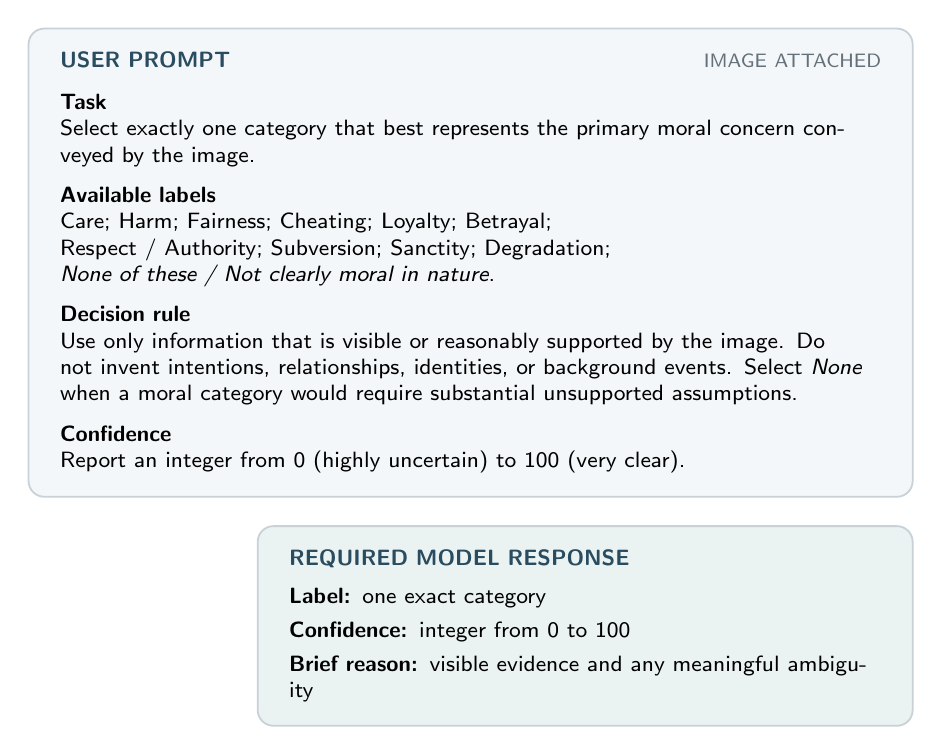
\begin{tikzpicture}[
    font=\sffamily\footnotesize,
    userbubble/.style={
        draw=promptRule,
        fill=promptUser,
        rounded corners=2mm,
        line width=.65pt,
        text width=.86\textwidth,
        align=left,
        inner xsep=4mm,
        inner ysep=3mm
    },
    modelbubble/.style={
        draw=promptRule,
        fill=promptModel,
        rounded corners=2mm,
        line width=.65pt,
        text width=.62\textwidth,
        align=left,
        inner xsep=4mm,
        inner ysep=3mm
    }
]

\node[userbubble] (prompt) {
    {\bfseries\color{promptNavy} USER PROMPT}
    \hfill
    {\color{promptMuted}\scriptsize IMAGE ATTACHED}\\[2mm]

    \textbf{Task}\\
    Select exactly one category that best represents the primary moral
    concern conveyed by the image.\\[1.8mm]

    \textbf{Available labels}\\
    Care; Harm; Fairness; Cheating; Loyalty; Betrayal;\\
    Respect / Authority; Subversion; Sanctity; Degradation;\\
    \textit{None of these / Not clearly moral in nature}.\\[1.8mm]

    \textbf{Decision rule}\\
    Use only information that is visible or reasonably supported by the
    image. Do not invent intentions, relationships, identities, or background
    events. Select \textit{None} when a moral category would require
    substantial unsupported assumptions.\\[1.8mm]

    \textbf{Confidence}\\
    Report an integer from 0 (highly uncertain) to 100 (very clear).
};

\node[modelbubble, anchor=north east] (response)
    at ([yshift=-3.5mm]prompt.south east) {
    {\bfseries\color{promptNavy} REQUIRED MODEL RESPONSE}\\[1.5mm]

    \textbf{Label:} one exact category\\[1mm]
    \textbf{Confidence:} integer from 0 to 100\\[1mm]
    \textbf{Brief reason:} visible evidence and any meaningful ambiguity
};

\end{tikzpicture}
\end{spacing}

\caption{Abridged illustration of the shared prompt used for primary
inference. The complete prompt is reproduced in
Appendix~\ref{app:prompt}.}
\label{fig:primary_prompt}
\end{figure}

Each model returned one moral-category label, one model-reported confidence
score, and one brief reason for every image. Confidence was treated as a
model-reported score rather than a calibrated probability. The brief reasons
were used to interpret category selections and disagreement cases, but not as
direct evidence of internal reasoning or classification correctness.

\subsection{Repeated-Run Stability Test}
\label{subsec:stability_design}

To assess stability within RQ2, each model classified the same stratified
32-image subset in three repeated runs using the common prompt reproduced in
Appendix~\ref{app:repeat_prompt}. The subset
included cases of both initial agreement and disagreement, allowing the
analysis to examine whether each model reproduced its own labels and whether
inter-model differences persisted across runs. Unlike the primary inference
stage, temperature zero was explicitly requested for all three models in these
repeat runs. Because the subset was purposively selected, the results describe
stability on these cases rather than across the complete corpus.

\section{Human Participant Survey}
\label{sec:human_survey}

\subsection{Survey Administration and Structure}
\label{subsec:survey_sample}
\label{subsec:survey_structure}

The questionnaire was administered online through
\href{https://qualtrics.ucl.ac.uk/jfe/form/SV_2aanTCkqVUzUcMC}{Qualtrics}.
Participants were recruited primarily through SurveySwap, with additional
recruitment through the researcher's personal network. Participation was
voluntary, restricted to adults aged 18 or over, and based on informed
consent. 

Recruitment produced a self-selected convenience sample, and no demographic
variables were collected. Before analysis, Survey Preview records and
incomplete records containing no substantive responses were excluded
\cite{eysenbach2004cherries}.

\subsection{Part 1: Moral-Category Selection}
\label{subsec:survey_part1}

Part~1 used a fixed pool of 16 images selected before the primary model
inference. The researcher first selected approximately one image considered
illustrative of each task category, and then randomly selected several
additional images from those considered either non-moral or potentially
morally meaningful. The pool was designed to cover the task categories and
include ambiguous cases; it was not intended to be a representative sample of
the full corpus. Restricting the pool to 16 images also kept the questionnaire
manageable, because asking each respondent to classify all 127 images would
have imposed excessive participant burden. Qualtrics randomly displayed five
images from this pool to each respondent.

For each image, respondents could select one or more of the same eleven
categories used in the model task. Allowing multiple selections enabled them
to express ambiguity or identify more than one relevant moral concern.
Responses were therefore analysed as category sets rather than as single
ground-truth labels. The image-pool identifiers, exact participant-facing
category definitions, and display logic are provided in
Appendix~\ref{app:survey_supplement}.


\subsection{Part 2: Supplementary Social-Level Ratings}
\label{subsec:survey_part2}

Part~2 contained nine supplementary items grouped into individual,
intergroup, and institutional dimensions. Qualtrics randomly displayed two of
the three items in each dimension, giving six ratings per respondent. Each
item used a five-point scale or a \textit{Not Applicable} option. These
exploratory ratings were analysed separately from the main moral-category
task. The exact question stems, image groups, response options, and display
logic are provided in
Appendix~\ref{app:part2_results}.

\section{Exploratory Matched Image-Edit Case Study}
\label{sec:visual_cue_sensitivity}

The aggregate comparisons showed whether the models agreed or disagreed, but
did not indicate which visible elements of an image might be associated with
their classifications. An exploratory matched image-edit case study was
therefore conducted to examine whether model labels and reported confidence
changed when selected visual cues were modified. The aim was to provide
case-level evidence about the visual information to which the models'
outputs appeared sensitive, rather than to identify their internal reasoning
mechanisms.

After the primary model runs, eight base images were purposively selected from
agreement and disagreement cases. Eleven edited variants were created in Adobe
Photoshop by modifying potentially relevant visual information, including
facial expression, body visibility, visible text, group composition, and
background context. Some base images contributed more than one variant.

Each variant was evaluated by all three models using the same classification
task as in the primary analysis. Its category label, model-reported confidence,
and brief reason were then compared with those of the corresponding base
image. Because an edit could alter more than one aspect of an image, observed
changes could not be attributed exclusively to the intended visual cue.
Moreover, the base outputs came from the primary runs whereas the variants
were evaluated in a later inference block, so ordinary between-call or
provider-side variation could also contribute to a difference. The cases were
therefore analysed descriptively rather than as controlled tests of causal
effects.

\section{Exploratory Prompt-Robustness Check}
\label{sec:prompt_robustness_design}

An exploratory robustness check tested whether alternative prompt instructions
changed how closely model labels corresponded with the participant selections
in RQ3. All three models classified the same 16 survey images under three
conditions built from a common prompt. P0 added no decision procedure; P1 and
P2 each added a different procedure:

\begin{center}
\small
\begin{tabular}{@{}p{0.14\textwidth}p{0.76\textwidth}@{}}
\toprule
\textbf{Condition} & \textbf{Difference from the common baseline} \\
\midrule
\textbf{P0} & Fresh baseline calls using the shared prompt prefix and common
suffix, with no additional decision procedure. \\
\textbf{P1} & The common prompt plus a structured procedure that separated
observation from interpretation, compared the leading category with an
alternative and \textit{None}, and calibrated confidence to the visible
evidence. \\
\textbf{P2} & The common prompt plus a separate cue-guided procedure that
prioritised direct and converging evidence and constrained inferences from
ambiguous cues, text, background, demographic composition, or unavailable
content. \\
\bottomrule
\end{tabular}
\end{center}

P1 and P2 were parallel, non-cumulative variants; P2 did not include the P1
procedure. P2 was derived from five image-edit families that did not include
any evaluation image, without using the survey targets or evaluation results.
Within each model, all three conditions used the same labels, confidence scale,
output fields, and request settings. P0 comprised new calls rather than the
retained RQ3 outputs.
The exact P1 and P2 additions are reproduced in
Appendix~\ref{app:repeat_prompt}.

\section{Analytical Measures}
\label{sec:analysis}

Without independently validated reference labels, the descriptive analyses
measured output patterns and agreement rather than accuracy or
population-level performance.


\subsection{RQ1: Overall Classification Patterns}

For image \(i\) and model \(m\), let \(y_{im}\) be the returned category and
\(\mathcal{C}_{M}\) the ten moral-category labels. Category and moral-label
selection rates were

\begin{equation}
    p_m(c)
    =
    \frac{1}{127}
    \sum_{i=1}^{127}
    \mathbb{I}\!\left(y_{im}=c\right),
    \qquad
    p_m^{(M)}
    =
    \sum_{c\in\mathcal{C}_{M}}p_m(c).
\end{equation}

\(p_m(c)\) is the proportion assigned to category \(c\), and \(p_m^{(M)}\) the
proportion assigned any moral label rather than \textit{None}. They describe
this fixed, uneven corpus rather than general model preferences.

Confidence was summarised by its mean, standard deviation, median,
interquartile range, range, and number of distinct values, then compared
between moral-label and \textit{None} outputs and across categories with at
least five observations. It was treated as an uncalibrated model-reported
score, not correctness. As a supplementary comparison, each model's outputs were also compared with
the researcher's working labels at the same eleven-label, six-outcome, and
binary resolutions. Raw agreement and unweighted Cohen's \(\kappa\) described
correspondence, while directional moral-label/\textit{None} counts showed
whether a model crossed the moral boundary more or less often than the
researcher. Because the working labels came from one researcher and were not
independently validated, these measures were not interpreted as accuracy.


\subsection{RQ2: Inter-Model Agreement and Repeated-Run Stability}
\label{subsec:inter_model}

Agreement at the eleven-label, six-outcome, and binary resolutions defined in
Section~\ref{subsec:category_framework} located disagreement at the exact
label, foundation, or moral-label/\textit{None} level. With \(g_r(\cdot)\)
denoting recoding at \(r\in\{11,6,2\}\), pairwise raw agreement was

\begin{equation}
A_{mm'}^{(r)}
=
\frac{1}{127}
\sum_{i=1}^{127}
\mathbb{I}\!\left[
g_r(y_{im})=g_r(y_{im'})
\right].
\end{equation}

\(A_{mm'}^{(r)}\) is the proportion of images receiving the same outcome.
Unweighted Cohen's \(\kappa\) accounted for marginal frequencies
\cite{cohen1960coefficient}, and exact three-model agreement was also
reported. Coarser agreement does not imply better performance.

To exclude agreement produced by shared \textit{None} outputs, images on which
both models selected a moral category were defined as

\begin{equation}
\mathcal{M}_{mm'}
=
\left\{
i:
y_{im}\in\mathcal{C}_{M}
\text{ and }
y_{im'}\in\mathcal{C}_{M}
\right\}.
\end{equation}

and conditional exact-label agreement as

\begin{equation}
A_{mm'}^{(11\mid M,M)}
=
\frac{1}{|\mathcal{M}_{mm'}|}
\sum_{i\in\mathcal{M}_{mm'}}
\mathbb{I}\!\left[
y_{im}=y_{im'}
\right].
\end{equation}

This measures specific-category agreement once both models selected a moral
label. Directional moral-label/\textit{None}, three-way, and within-foundation
differences, together with confidence and selected cases, located the remaining
disagreements.

For the 32-image repeat subset, let \(y_{imt}\) be the label for image \(i\),
model \(m\), and run \(t\in\{1,2,3\}\). Mean within-model agreement was

\begin{equation}
R_m^{(r)}
=
\frac{1}{3}
\sum_{1\leq a<b\leq3}
\left[
\frac{1}{32}
\sum_{i=1}^{32}
\mathbb{I}\!\left[
g_r(y_{ima})=g_r(y_{imb})
\right]
\right],
\qquad r\in\{11,6,2\}.
\end{equation}

\(R_m^{(r)}\) averages the three run pairs and therefore measures within-model
stability. Run-pair ranges, three-run unanimity, and Fleiss' \(\kappa\)
\cite{fleiss1971measuring} supplemented it; corresponding rounds were compared
between models using raw agreement and Cohen's \(\kappa\).

For images \(\mathcal{U}_m\) with a unique modal repeat label
\(\widetilde{y}_{im}\), let \(y_{im}^{(0)}\) be the primary classification.
Primary-to-repeat continuity was

\begin{equation}
C_m^{(r)}
=
\frac{1}{|\mathcal{U}_m|}
\sum_{i\in\mathcal{U}_m}
\mathbb{I}\!\left[
g_r(y_{im}^{(0)})
=
g_r(\widetilde{y}_{im})
\right].
\end{equation}

\(C_m^{(r)}\) measures whether primary classifications matched the modal repeat
labels. It was termed \textit{continuity} because the two blocks used
non-identical settings. Modal-label agreement between models was also reported;
all repeat results apply only to the selected subset.

\subsection{RQ3: Participant Variation and Participant--Model Correspondence}
\label{subsec:human_model_support}

Let \(H_{ij}\) be respondent \(j\)'s category set for image \(i\), and \(N_i\)
the number shown that image. Category endorsement was

\begin{equation}
    E_i(c)
    =
    \frac{1}{N_i}
    \sum_{j=1}^{N_i}
    \mathbb{I}\!\left(c\in H_{ij}\right).
\end{equation}

\(E_i(c)\) is the proportion selecting \(c\); because responses were
multi-label, an image's proportions could sum to more than one.

The categories maximising \(E_i(c)\) formed the plurality set. For the
supplementary top-two comparison, let \(\mathcal{C}\) be the eleven categories,
\(n_i(c)\) the count selecting \(c\), and

\begin{equation}
    R_i(c)
    =
    1+
    \sum_{d\in\mathcal{C}}
    \mathbb{I}\!\left[n_i(d)>n_i(c)\right].
\end{equation}

define

\begin{equation}
    \mathcal{T}_i^{(2)}
    =
    \left\{
        c\in\mathcal{C}:
        n_i(c)>0,
        \ R_i(c)\leq2
    \right\}.
\end{equation}

\(\mathcal{T}_i^{(2)}\) includes positive-count categories ranked first or
second, retaining ties. Membership of a model label measured top-two
correspondence; plurality membership was the stricter comparison. Neither was
treated as correctness.

Participant endorsement of model \(m\)'s selected category was

\begin{equation}
    S_i^{(m)}
    =
    E_i(y_{im}).
\end{equation}

\(S_i^{(m)}\) is the proportion who included the model-selected category.

Overall endorsement was

\begin{equation}
    S_{\mathrm{macro}}^{(m)}
    =
    \frac{1}{16}
    \sum_{i=1}^{16}
    S_i^{(m)},
    \qquad
    S_{\mathrm{micro}}^{(m)}
    =
    \frac{
        \sum_{i=1}^{16}N_iS_i^{(m)}
    }{
        \sum_{i=1}^{16}N_i
    }.
\end{equation}

The macro average weights images equally; the micro average weights their
response counts, showing whether unequal presentation affected the summary.
Descriptive percentile bootstrap intervals resampled images for the former and
respondents as clusters for the latter \cite{efron1993bootstrap}.

Within-image participant similarity used the Jaccard coefficient
\cite{jaccard1912distribution}:

\begin{equation}
    J_i(j,k)
    =
    \frac{
        |H_{ij}\cap H_{ik}|
    }{
        |H_{ij}\cup H_{ik}|
    }.
\end{equation}

Higher values indicate more similar sets. Values were averaged within images
and then equally across the 16 images; category counts described response
breadth. Pearson and Spearman correlations tested whether confidence tracked
endorsement, without treating this as calibration. A sensitivity check removed
\textit{None} from responses that also contained a moral category.


\subsection{RQ4: Image-Edit Case Measures}

For valid variants \(V_m\), with \(b(v)\) denoting the matched base image, the
label-change rate was

\begin{equation}
    L_m
    =
    \frac{1}{|V_m|}
    \sum_{v\in V_m}
    \mathbb{I}\!\left[
        y_{vm}^{(\mathrm{variant})}
        \neq
        y_{b(v)m}^{(\mathrm{base})}
    \right],
\end{equation}

\(L_m\) measures how often an edit was followed by a different label. For
model-reported confidence \(q\), paired change was

\begin{equation}
    \Delta q_{vm}
    =
    q_{vm}^{(\mathrm{variant})}
    -
    q_{b(v)m}^{(\mathrm{base})}.
\end{equation}

Positive values indicate increased confidence after editing and negative
values a decrease. Mean, median, interquartile range, and range summarised these
changes. Together with edit type and brief reasons, the two measures described
exploratory sensitivity rather than isolated causal effects.


\subsection{Supplementary Survey Part 2 Measures}
\label{subsec:survey_part2_analysis}

Part~2 items were reported separately using valid sample size, mean, standard
deviation, median, and interquartile range; \textit{Not Applicable} was
excluded, and no composite or inferential comparison was used because the
items did not form a validated scale.

\section{Implementation, Data Management, and Ethical Considerations}
\label{sec:implementation}

\subsection{Analysis Implementation}

Image identifiers, model outputs, and survey responses were processed in Python
and linked by file stem. Each component used its retained source: the primary
model files, screened Qualtrics export, stability manifest and repeat records,
or explicit base--variant mapping. The researcher performed screening, linkage,
statistical analysis, and interpretation; API credentials were excluded from
analysis and sharing materials. The file inventory and reproducibility
information appear in Appendix~\ref{app:reproducibility}.


\subsection{Ethical Considerations and Data Handling}
\label{sec:ethical_considerations}

An ethics application for this study has been submitted to the university.

Some corpus images depicted potentially sensitive social or moral situations.
The online-source images were reusable open-source materials, and the remainder
were generated for the project with Google Gemini, as described in
Section~\ref{subsec:image_collection}. Only image files needed for inference,
never participant survey records, were submitted to hosted provider APIs.

Survey participation was voluntary and limited to adults aged 18 or over. The
information page explained the study and stated that selecting \textit{Next}
indicated consent. The questionnaire used Qualtrics' anonymous-link mode and
requested no names, contact details, demographic information, or other direct
identifiers.

The restricted export retained platform response identifiers, timestamps, and
network-derived metadata, accessible only to the researcher under access
control. These technical fields were removed before analysis. Public materials
contain only aggregated, non-identifiable results; retention and deletion will
follow the arrangements described in the submitted ethics application, the
participant information, and applicable university data-management requirements.
